\chapter{Implementazione}
\label{capitolo5}
\thispagestyle{empty}



\noindent All'interno di questo capitolo verranno illustrate tutte le tecniche implementative per realizzare quanto è stato enunciato nel capitolo precedente. Nel dettaglio verranno spigate, argomentate le implementazioni effettuate su tutte le fasi della tesi, i riferimenti teorici che hanno permesso la realizzazione di questa tesi.
\section{Raccolta dati}
La raccolta dati è la fase iniziale della tesi di laurea. Come precedentemente argomentato il social network di riferimento utilizzato è \textit{Twitter}.Prima di spiegare quanto fatto occorre citare le funzionalità della \textit{Twitter Api}. Successivamente verranno illustrate le tecniche adottate per la raccolta dei \textit{Tweet} del passato.
\subsection{Twitter Api}
Sono delle api messe a disposizione dal social network Twitter, per poterle utilizzare occorre necessariamente effettuare l'iscrizione al reparto sviluppatori di Twitter, mettendo a disposizione il proprio account personale, quindi come prima cosa occorre predisporre di un proprio account. La raccolta dei dati può essere effettuata soltanto dopo aver abilitato l'account. Per raccogliere i dati pubblicati dagli utenti all'interno della rete occorre creare una \textit{Twitter Apps}, la quale rilascerà delle credenziali che dovranno essere utilizzate per poter effettuare le richieste attraverso le Twitter Api al server. Viene inizializzato un processo di streaming tra il client ed il server che consenta la ricezione dei dati, diamo una definizione delle credenziali, che sono divise in:
% Tale operazione viene eseguita attraverso un processo di streaming, questa operazione occorre creare una \textit{Twitter Apps} il quale rilascerà una volta creata una serie di codici che dovranno essere utilizzati per poter effettuare le richieste con le Twitter Api al server.
%Le credenziali sono divise in:
\begin{itemize}
\item \textit{Token}: identificano il token di accesso ai servizi messi a disposizione da Twitter, a sua volta è composto da:
\begin{itemize}
\item \textit{Access token}
\item \textit{Access secret}
\end{itemize}
\item \textit{Consumer}: è un codice di accesso ai servizi di consumo, ovvero consente lo streaming dei dati dal server, si suddivide in due chiavi:
\begin{itemize}
\item \textit{Consumer key}
\item \textit{Consumer secret}
\end{itemize}
\end{itemize}
Queste chiavi di accesso possono essere generate più e più volte, una volta creata un'applicazione per lo sviluppo di Twitter.
Le Api sono disponibili in diversi linguaggi di programmazione tra cui il \textit{Python}, utilizzato per lo sviluppo della tesi.
Per richiamare tutte le api attraverso il codice è necessario sempre autenticarsi, caricando le credenziali di accesso  fornite attraverso i permessi da sviluppatore precedentemente illustrate.
Lo streaming per la raccolta dei dati è soggetto a stringenti regole per evitare un uso improprio delle informazioni diffuse dagli utenti all'interno della rete. Infatti c'è un numero massimo di richieste che un utente, con le credenziali da sviluppatore, può effettuare, cioè 100 ogni 15 minuti. Allo scadere di tale tempo potrà ricominciare, altrimenti nel caso in cui un utente non tenesse conto di questa limitazione ed effettuasse una nuova richiesta durante il tempo di pausa le sue credenziali verrebbero bloccate per circa un'ora non potendo più interagire con le api di Twitter.
La risposta da parte del server sarà un file \textit{JSON} contenente tutti i metadati dell'utente in questione, come il testo del Tweet, il suo id, lo username dell'utente che ha effettuato il tweet, i mentions gli hashtag ed il numero di retweet con la lista degli utenti che hanno retwettato la notizia in questione.

\subsection{Get Old Tweet}
Questa sezione illustrerà in che modo sono stati raccolti tutti i tweet del passato. Avendo spiegato nella sezione precedente le problematiche relative al numero di richieste da effettuare nell'arco temporale, è stata seguito un approccio differente che consentiva di limitare il numero di richieste alla volta.
L'approccio in questione consiste nell'effettuare una \textit{GET} sulla pagina di ricerca di Twitter, specificando l'argomento ricercato, ed il periodo di validità della ricerca.
Twitter suddivide gli account abilitati allo sviluppo in 3 categorie:
\begin{itemize}
\item \textit{Standard}: account gratuito soggetto a limitazione temporali e sui contenuti, non è possibile ricercare tweet precedenti a 7 giorni. I dati richiesti non sono completi.
\item \textit{Premium}: account a pagamento con sole limitazioni temporali, non è possibile ricercare tweet precedenti a 30 giorni. Non ha nessun problema di completezza sui contenuti.
\item \textit{Enterprise}: account a pagamento senza alcuna limitazione temporale e sui contenuti.
\end{itemize}
Avendo utilizzato un account \textit{Standard} sono stati ricercati dei metodi per poter risolvere le problematiche precedentemente descritte, cercando di ottenere più informazioni possibili.
%Un altro problema che ha spinto all'utilizzo di questo metodo riguarda la politica di Twitter nel far collezionare, agli utenti non premium con i permessi di sviluppo, soltanto i dati con data di riferimento di 7 giorni precedenti alla data di ricerca selezionata. Per di più come indicato all'interno della documentazione i dati raccolti mediante le Twitter Api non saranno tutti quelli pubblicati nel periodo selezionato.

Tutte queste problematiche sono state risolte la libreria \textit{Get Old Tweet}, il quale crea un indirizzo http con i parametri di ricerca richiesti, nel nostro caso:
\begin{itemize}
\item \textit{La query}: la parola chiave, l'hashtag da ricercare all'interno dei Tweet.
\item \textit{Data inizio}: la data in cui inizio a raccogliere i dati.
\item \textit{Data Fine}: la data in termino la ricerca e la raccolta dei dati.
\end{itemize}
Una volta definiti questi parametri all'interno della \textit{url}, viene restituita la pagina html contenente tutti i  tweet presenti nel periodo indicato. Il risultato verrà convertito in un formato \textit{json}, per estrarre le informazioni basterà parsare la pagina ottenendo i seguenti dati:
\begin{itemize}
\item Lo \textit{username} della persona che ha postato il tweet.
\item Il numero di \textit{retweet} al tweet. 
\item Il \textit{testo} del tweet pubblicato.
\item La lista  degli \textit{hashtag} pubblicati dall'utente all'interno del tweet
\item La lista dei \textit{mentions} pubblicati dall'utente all'interno del tweet.
\item La \textit{data} di pubblicazione del tweet.
\end{itemize}
Per far comprendere meglio queste informazioni nell'immagine sovrastante viene presentato un tweet di esempio con le informazioni precedentemente elencate, per far comprendere al meglio gli elementi in questione.
\begin{figure}[h]
    \begin{center}
      
\includegraphics[scale= 0.8]{trump.png}
	%
\psfig{file=./pictures/logo}
	\caption{esempio Tweet}
    \end{center}
  \end{figure}
  
Tutti questi dati sono stati successivamente elaborati ed analizzati. Particolare attenzione è stata posta a due di essi ovvero: il testo ed il numero di retweet. 
Il primo per effettuare la sentiment analysis e poter definire una prima partizione dei dati, che andranno a generare il grafo.
Il secondo perché costituisce la base per i nuovi nodi del grafo e quindi la diffusione del tweet con altri utenti. 
Per identificare la lista degli utenti che hanno effettuato il retweet sul tweet in questione è stato necessario usare una libreria chiamata \textbf{Tweepy}.
Questa libreria sfrutta le \textit{Twitter Api}, effettuando delle chiamate rest sul server di Twitter per ricevere le informazioni richieste. Nel nostro caso è stato utilizzato il metodo \textit{retweet} che ricevendo come argomento l'id relativo al tweet pubblicato permette di ricevere la lista degli username che hanno pubblicato quell'argomento all'interno della propria rete. Il problemi presentati in precedente nell'utilizzare queste chiamate al server sono sempre validi, infatti se vengono superate le 100 richieste viene lanciata un'eccezione: \textit{Tweepy Error} che consente di mettere in pausa l'applicazione attraverso una sleep per 15 minuti. Una volta terminato il tempo di attesa la richiesta viene ripresa dal punto richiesto, continuando a collezionare gli username richiesti.
Tutti i dati raccolti durante le operazioni di streaming sono stati salvati all'interno di un file binario per poter ottimizzare lo spazio fisico.

\subparagraph{EC2}
La raccolta dati utilizzando le implementazioni precedentemente citate, è stata eseguita all'interno di una istanza \textbf{EC2}. 
Il motivo di tale scelta è dettata dai tempi di attesa via via sempre più lunghi per la raccolta degli username degli utenti che hanno retweettato i tweet raccolti, per via delle politiche stringenti dettate da \textbf{Twitter}.  Utilizzando un'istanza a pagamento, si è dovuto ottimizzare il salvataggio fisico dei dati, perché oltre ad essere un servizio a consumo di risorse di calcolo, vengono pagate anche i dati salvati all'interno dello storage fisico della macchina. Attraverso la libreria \textit{pickle}\footnote{libreria per il salvataggio dei dati fornita da \textit{Python}} si è potuto risolvere questo problema, in quanto ottimizza il salvataggio dei dati attraverso una conversione in binario degli stessi.


\section{Sentiment Analysis}
La sentiment analysis è l'approccio utilizzato per la divisione dei diversi tweet, raccolti per un determinato topic, analizzando il "sentimento" espresso nel contenuto del testo pubblicato dagli utenti.
Questa fase viene effettuata al momento della raccolta dei dati, cioè una volta collezionati l'insieme dei dati vengono sottoposti alla funzione implementata e salvati in due categorie distinte mediante la libreria \textit{pickle}, precedentemente illustrata.

L'implementazione di questo metodo è stata effettuata seguendo un approccio basato su \textit{metodi statistici}: questi metodi si basano su elementi di apprendimento automatico. Per misurare l'opinione nel contesto e trovare la caratteristica che è stata giudicata, sono usate le relazioni grammaticali delle parole utilizzate. Le relazioni di dipendenza grammaticale sono ottenute attraverso la scansione approfondita del testo. Il processo di apprendimento da parte della macchina (anche detto machine learning) non è immediato, devono infatti essere costruiti dei modelli che associano a diverse tipologie di commenti una polarità e se necessario ai fini dell'analisi anche un topic.

Si può riassumere quanto sviluppato attraverso la seguente immagine:
\begin{figure}[!h]
    \begin{center}
      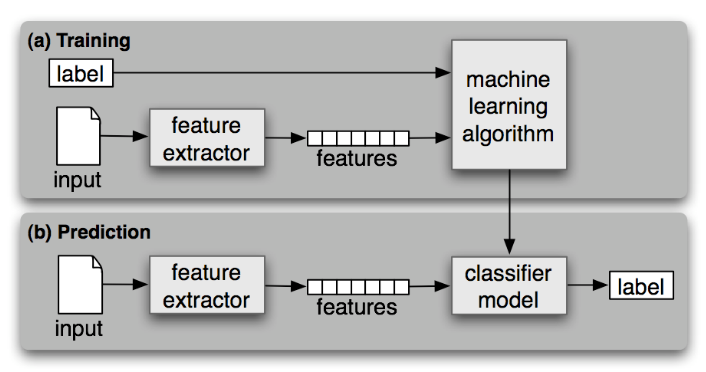
\includegraphics[scale= 0.55]{sentiment.png}
	%
\psfig{file=./pictures/logo}
	\caption{schema Sentiment Analysis}
    \end{center}
  \end{figure}
 
 Da quanto si evince dall'immagine mostrata risulta evidente quanto un meccanismo di \textit{machine learning} necessiti di un classificatore molto preciso. La precisione può essere ottenuta attraverso dei \textit{training set}, ovvero dei file che istruiscano la macchina permettendo una classificazione ottimale dei dati.
Ci sono diversi classificatori, quello utilizzato per l'implementazione della Sentiment Analysis è descritto di seguito.
\begin{itemize}
\item \textbf{classificatore Naive Bayes}:
Un classificatore bayesiano è un classificatore basato sull'applicazione del teorema di Bayes.
Richiede la conoscenza delle probabilità a priori e condizionali relative al problema, quantità che in generale non sono note ma sono tipicamente stimabili. Se è possibile ottenere delle stime affidabili delle probabilità coinvolte nel teorema, il classificatore bayesiano risulta generalmente affidabile e potenzialmente compatto. Per costruzione, il classificatore bayesiano minimizza il rischio di classificazione.

Nel gergo della classificazione di testi o \textit{Text Categorization}, con il termine classificatore bayesiano ci si riferisce convenzionalmente al classificatore Naive Bayes, ossia un classificatore bayesiano semplificato con un modello di probabilità sottostante assume l'indipendenza delle \textit{feature}, ovvero che la presenza o l'assenza di una particolare \textit{feature} in un documento testuale non è correlata alle altre.

L'esperienza dimostra che il metodo funziona in molti problemi pratici, come per esempio il filtraggio antispam adattivo. Un vantaggio del classificatore Naive Bayes è che richiede solo un training set di esigue dimensioni per stimare i parametri necessari per la classificazione

\end{itemize}

Tornando allo sviluppo, la prima operazione fatta è stata quella di raccogliere dati per classificare i tweet secondo un determinato topic. Questa operazione è stata effettuata manualmente anche per per permettere alla macchina di poter riconoscere l'ironia. Attraverso un file csv\ref{training} costruito con due colonne:
\begin{itemize}
\item \textit{label}: ovvero l'identificatore che verrà utilizzato nell'analisi del classificatore per analizzare il contenuto di tweet ed associarlo ad un gruppo piuttosto che ad un altro.
\item \textit{Tweet}: il testo del tweet pubblicato, contenente anche caratteri speciali, elementi multimediali, link etc.
\end{itemize}
%Inserire una tabella con un esempio dei tre valori
\begin{table}
\centering

\begin{tabular}{ |p{3cm}||p{7cm}| }
 \hline
 \multicolumn{2}{|c|}{Training set} \\
 \hline
 Label & Tweet\\
 \hline
 5stelle   & Chi ama la sua terra non può che votare il \#M5S \#Regionali \#Sicilia pic.twitter.com/gv3CQWhCeI   \\
 ForzaItalia &   Con elezioni $ @matteosalvinimi$ e $@Musumeci\_Staff$ regionali 2017 in \#Sicilia !!\#elezioniregionali2017 \#andiamoagovernare \#forzalega  \\
Altri & Tutti gli schieramenti alle \#elezioniregionali in Sicilia.L'articolo di Pierangelo Bonanno \\
 \hline
\end{tabular}
\label{training}
\caption{Esempio di training set}
\end{table}
Una volta definito un training set occorre definire un \textit{vettore di Feature}:
\begin{itemize}
\item Rappresenta l'elemento cardine di un classificatore, maggiore è la sua efficienza e maggiore sarà la precisione del classificatore. Il vettore di feature è utilizzato per costruire un modello che consenta al classificatore di poter apprendere attraverso un training set, di poter fare una predizione sui dati che non ha mai analizzato prima.
Dovendo analizzare dei dati basati su Twitter si è deciso di adottare degli schemi basati sull'assenza o meno di alcune parole che appaiono nei tweet come feature. Attraverso il training set, composto da tweet suddivisi in 3 gruppi (positivi, negativi e neutrali), suddividiamo ciascun tweet in parole e aggiungeremo ogni parola la vettore di feature. Tale approccio viene definito \textit{unigrams}.Prima di andare ad inserire tali parole all'interno di questo vettore andremo ad effettuare delle operazioni di filtraggio scartando quelle parole che non sono necessarie per comprendere il sentimento. 
Nel nostro caso le congiunzioni, articoli, preposizioni semplici ed articolate, ma anche altri caratteri perché generalmente i tweet contengono caratteri speciali come \textit{\# , @, link},  vengono inseriti all'interno della lista di parole di \textit{Stop}, cioè una lista popolata da tutte quelle parole che potrebbero far saturare il vettore di feature e che non esprimono un sentimento.
Il vettore di feature viene popolato a partire da tutte le parole che non sono presenti all'interno della lista di \textit{Stop} e che appartengono a tutti i tweet del training set.
\end{itemize}

 
In conclusione una volta definito il classificatore, il vettore di Feature ed il training set non resta che illustrare il calcolo della sentiment Analysis.
Per l'implementazione del classificatore \textit{Naive Bayes} si è utilizzata la libreria \textit{Python} \textbf{NLTK}\footnote{Natural Language Toolkit.}, la quale una volta istruito il classificatore attraverso il training set utilizza il vettore di feature per ricercare la vicinanza del tweet al traiining set, restituendo il label corrispettivo ( inserito dall'utente nella definizione del csv sopra citato).


